% Generated by run_paper_results.m; do not edit numerical values manually.
\subsubsection{Benchmark and implementation contract}
We regenerate the six-DG, seven-line benchmark using the component values and initial condition retained in the original MATLAB implementation. The plant has ZI loads and continuously varying resistive line currents. All reported controllers act on the same plant and equilibrium. The equilibrium enforces the voltage, command, exported-current, and proportional-current-sharing constraints in \eqref{Eq:DGSpecs1}--\eqref{Eq:DGSpecs4}.
The common current-utilization fraction is $0.531555$; equilibrium voltages range from $47.3536$ to $49.0523$ V. The maximum equilibrium equation residual is $5.41\times 10^{-11}$.
States and physical inputs are divided by 48, and time is normalized by $t_0=10^{-3}$ s. This common scaling of the two local states preserves the scalar-block supply parametrization. Local supplies use $\mathcal X_i=[a_i I,\,\frac12 I;\,\frac12 I,\,-\rho I]$ with $a_i>0$. The global performance bound is from the additive normalized state disturbance to the normalized state error, rather than directly from primitive current/voltage noise.
The shared tuning grid is $\rho\in\{0.15,0.2,0.25,0.28\}$; minimizing the worse certified gain of an accepted MB/DD pair selects $\rho=0.2$. The global gain bound is 20, the common transformed communication budget is 10, and the normalized distance-weighted $\ell_1$ penalty is 0.02. Failed tuning attempts are retained with solver diagnostics.
\subsubsection{Data-driven experiment and scope}
To avoid treating physical line currents as independent held inputs, the data-driven implementation uses an exact continuous-time integral regression. On each acquisition interval, let $X_i$ and $U_i$ contain the measured average state and average two-channel input, and let $\Delta_i$ contain the endpoint state difference divided by the normalized interval length. Then
\begin{equation}\Delta_i=\widetilde A_i X_i+\widetilde B_i U_i+W_i.\label{Eq:IntegralDataRegression}\end{equation}
Each DG supplies 400 transitions with a physical acquisition interval of $0.0001$ s. Converter commands are held on each interval, while the resistor network evolves continuously. A fixed local current-feedback gain of $-1$ is supplemented by independent uniform excitation of amplitude 0.25 in normalized units. State and input measurements are noise-free. Primitive process disturbances are independently drawn in a box of Euclidean radius at most $d_{\max}=0.0001$ per DG.
Before generating the data, we declare $\|\widetilde B_i\|_2\leq 1.25$ and $W_iW_i^\top\preceq\eta I$, where $\eta=T(1.25 d_{\max})^2=6.25\times 10^{-6}$. This bound is not fitted to the realized residuals. All six input-state regression matrices have rank four, their data-consistency sets have strict interior, and independent checks confirm true-model membership and the integral data equation.
The product of local data-consistency sets is used as a conservative outer approximation, without an independence assumption on physical line-current data. Positive QMI scaling and a fixed invertible congruence improve numerical conditioning. The continuous-time local data certificate is implemented as the following sufficient S-procedure. Define
\begin{equation}N_i=\begin{bmatrix}\eta I-\Delta_i\Delta_i^\top&\Delta_i R_i^\top\\R_i\Delta_i^\top&-R_iR_i^\top\end{bmatrix},\qquad R_i=\begin{bmatrix}X_i\\U_i\end{bmatrix}.\end{equation}
With $P_i\succ0$, $L_i=[0;\ell_i]$, and $\lambda_i\geq0$, the implementation enforces the hard LMI \eqref{Eq:IntegralLocalCertificate}.
\begin{figure*}[t]\begin{equation}\begin{bmatrix}0&-P_i&-L_i^\top&\frac12P_i-I&P_i\\-P_i&0&0&0&0\\-L_i&0&0&0&0\\\frac12P_i-I&0&0&a_iI&0\\P_i&0&0&0&\rho^{-1}I\end{bmatrix}-\lambda_i\operatorname{diag}(N_i,0,0)\succeq0.\label{Eq:IntegralLocalCertificate}\end{equation}\hrulefill\end{figure*}
Substitution of $[e_i;\widetilde A_i^\top e_i;\widetilde B_i^\top e_i;v_i;q_i]$, followed by a Schur complement and congruence, gives the original continuous-time local storage inequality for $K_i=L_iP_i^{-1}$ and storage $P_i^{-1}$. Thus this experiment implements a sufficient continuous-time integral-data counterpart; it does not use a forward-Euler approximation of the physical network.
The data-driven local stage is followed by the hard model-based global composition LMI using the known input matrices and physical conductance network. Consequently, the DD results below are explicitly a local data-driven/known-input-matrix global design. They do not validate the general unknown-input-matrix global construction in Prop.~\ref{Pr:DataDrivenGlobalControllerDesign}, whose lifted LMI remains subject to the principal-block obstruction documented in the revision audit. No softened certificate is accepted. Every selected graph is imposed in a second solve, and the original local, global supply-dominance, and aggregate storage inequalities are checked independently after gain recovery.
\subsubsection{Regenerated responses and quantitative comparison}
As an external literature baseline, we implement the conventional decentralized voltage--current droop law $V_{ti}=V_{0i}-R_{di}I_{ti}$ used as a primary control layer in \cite{Guerrero2011HierarchicalDroop,Lu2014ImprovedDroop}. The coefficients are fixed before simulation as $R_{di}=\delta_V V_{\mathrm{rated},i}/I_{\mathrm{rated},i}$ with $\delta_V=5\%$, giving $R_{di}\in[0.1034,0.4397]$ $\Omega$. For a matched comparison, $V_{0i}=V_{Sti}+R_{di}I_{Eti}$ preserves the same verified equilibrium and feedforward command as the other methods. The controller uses only local converter current, has no communication links, and carries no dissipativity or robustness-certificate claim. It represents conventional primary droop, not the communication-based secondary restoration loops proposed in \cite{Lu2014ImprovedDroop}.
Figure~\ref{Fig:DCMG-Comparison} regenerates the original large-initial-error comparison using freshly synthesized controllers. These are linear-model responses: command saturation and independent line-current clipping are disabled. The archived initial condition includes negative voltages and large current errors, so this plot is a mathematical reproduction benchmark rather than an operating-envelope validation.
\begin{figure*}[t]\centering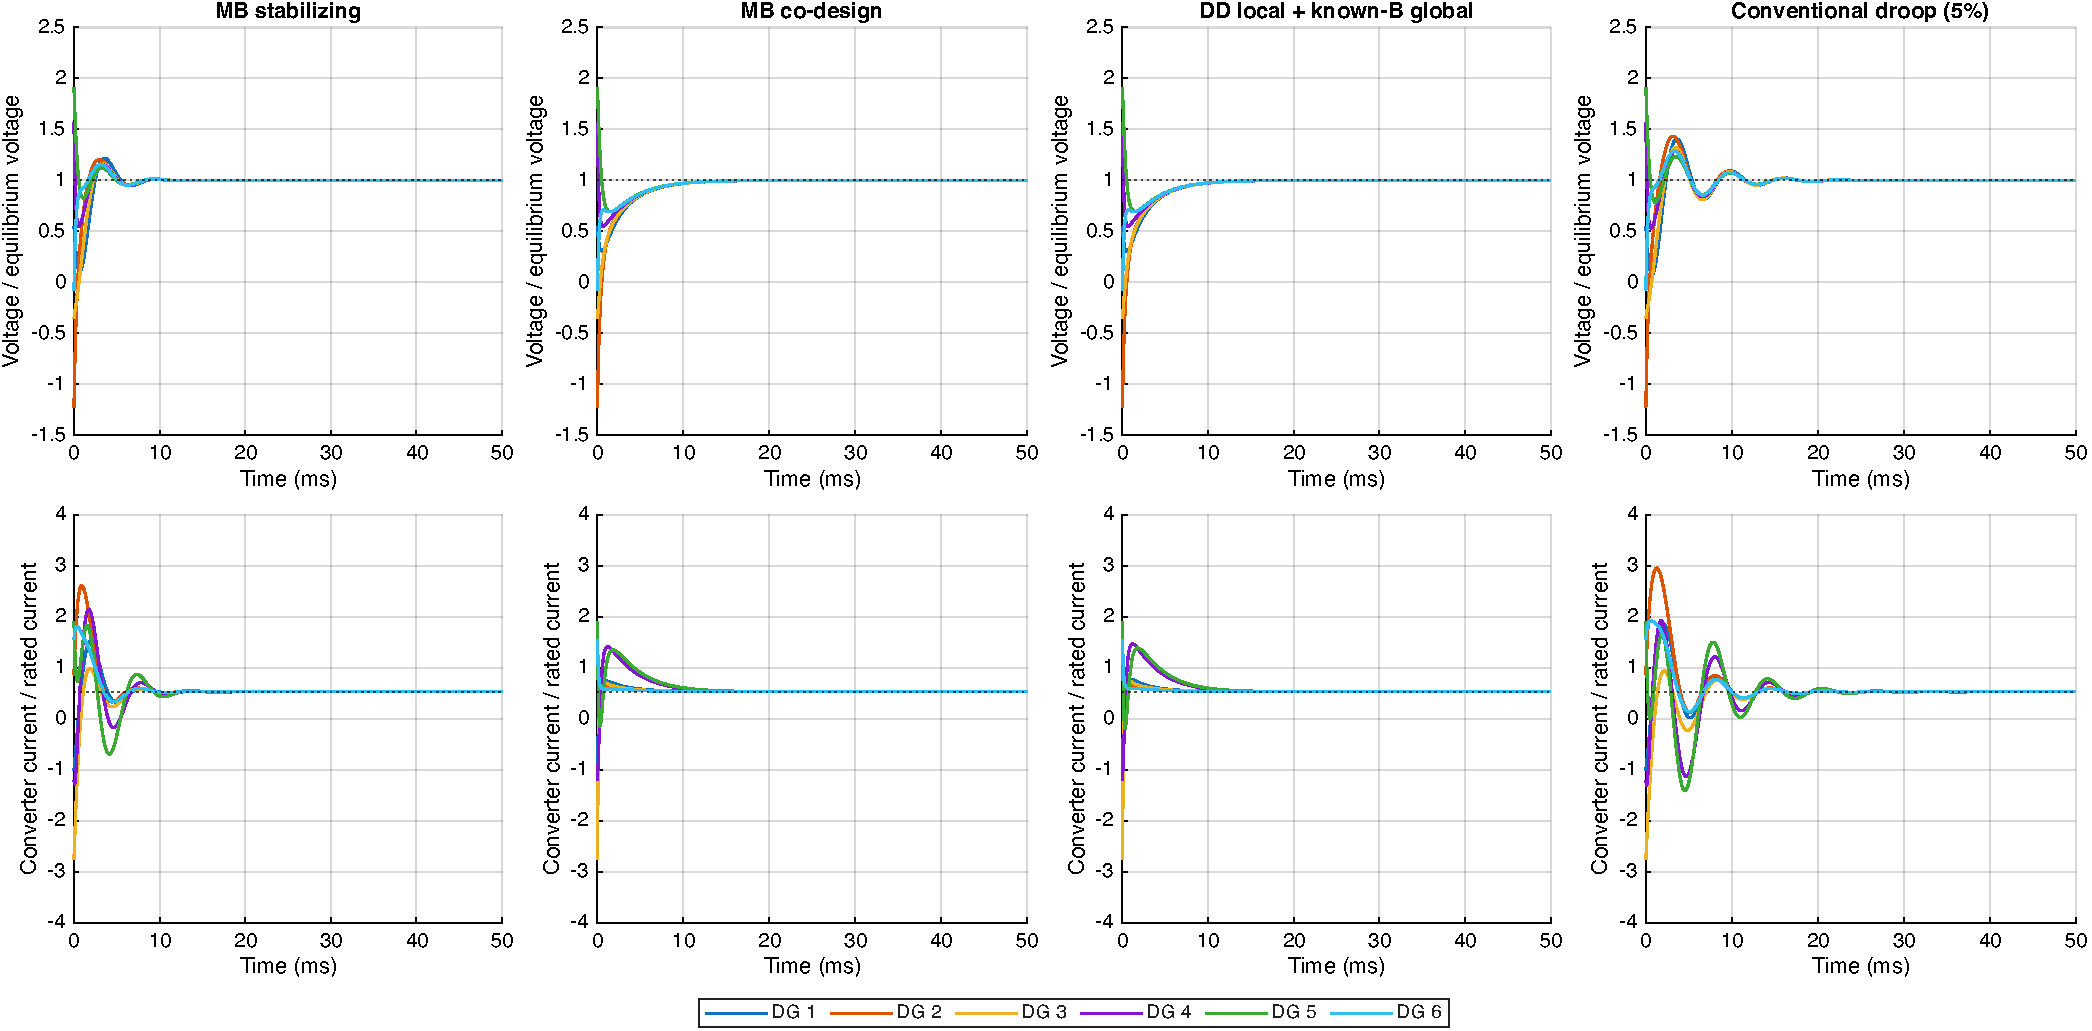
\includegraphics[width=0.99\textwidth]{Results/Regenerated/paper_trajectories.pdf}\caption{Fresh controller responses from the archived six-DG initial condition. Columns use the stabilizing MB, hierarchical MB, integral-data local/known-$B$ global, and conventional droop controllers.}\label{Fig:DCMG-Comparison}\end{figure*}
\begin{figure*}[t]\centering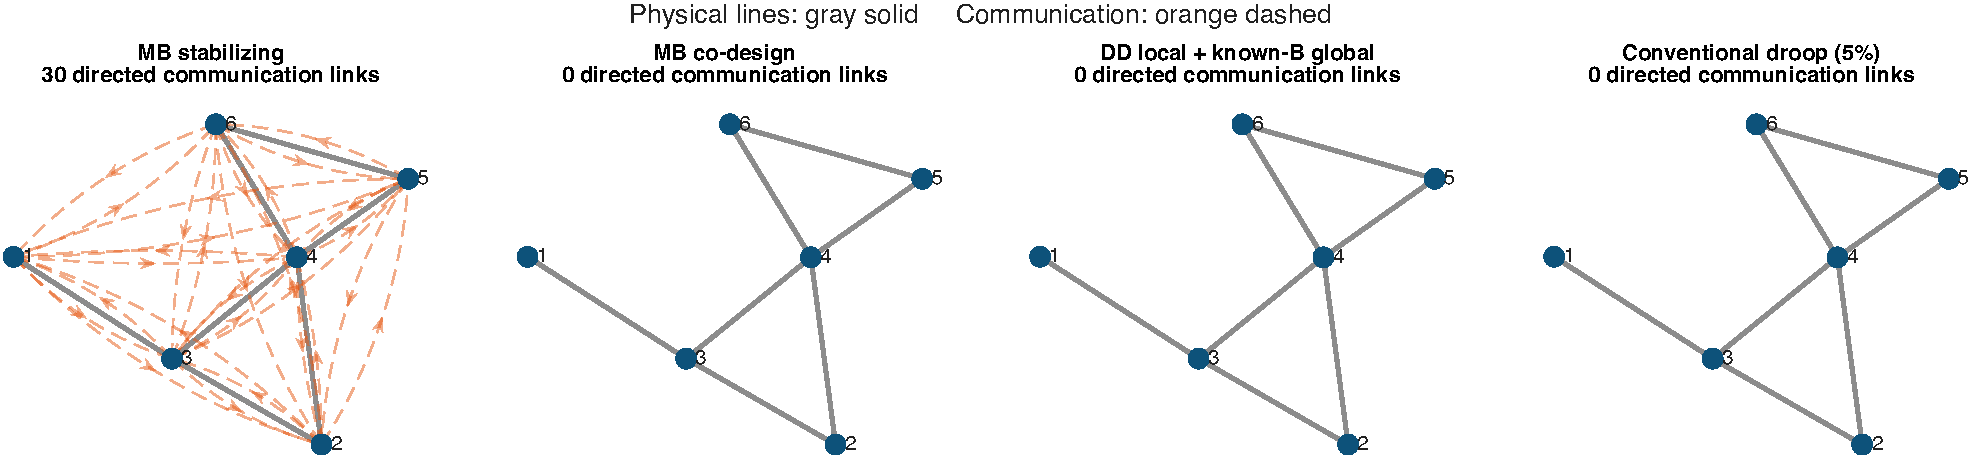
\includegraphics[width=0.96\textwidth]{Results/Regenerated/paper_topologies.pdf}\caption{Regenerated topologies. Gray solid edges are the seven physical resistive lines; orange dashed arrows are directed communication links. Local self-feedback is excluded from the communication count.}\label{Fig:RegeneratedTopologies}\end{figure*}
The stabilizing design uses 30 directed communication links. Both co-designs retain nonzero local and diagonal coordination feedback but require 0 and 0 off-diagonal links, respectively (Fig.~\ref{Fig:RegeneratedTopologies}). In this experiment the physical coupling and equilibrium feedforward allow the optimized feedback to be decentralized. This outcome supersedes the historical 15-link picture and should not be interpreted as a universal zero-communication result.
For the quantitative nominal comparison, initial voltage/current offsets are $\pm1.5$ V and $\pm0.35$ A with a fixed sign pattern. Settling time is the last-entry time into two percent of the initial normalized state-error norm. A separate, matched disturbance experiment starts at equilibrium, applies a fixed-sign current/command disturbance pulse of amplitudes 0.35 A and 0.5 V on 25--35 ms, and applies a symmetric state jump at 65 ms. The voltage and sharing RMS metrics in Table~\ref{Tab:RegeneratedMetrics} are evaluated over this complete 120 ms disturbance run.
\begin{table*}[t]\centering\caption{Recomputed metrics. The certified $\gamma$ uses normalized additive state disturbances. A dash denotes a non-certified comparison controller.}\label{Tab:RegeneratedMetrics}\begin{tabular}{lrrrrrr}\hline Method & Directed links & $\gamma$ & Max. Re pole & Settling (ms) & Voltage RMS (V) & Sharing RMS (p.u.)\\\hline
MB stabilizing & 30 & -- & -408.93 & 5.20 & 0.0750 & 0.01763 \\
MB co-design & 0 & 5.0872 & -315.55 & 3.30 & 0.1600 & 0.00339 \\
DD local / known-$B$ global & 0 & 5.0975 & -331.97 & 3.20 & 0.1520 & 0.00336 \\
Conventional droop (5\%) & 0 & -- & -213.63 & 6.30 & 0.1230 & 0.01663 \\
\hline\end{tabular}\end{table*}
On this fixed linear ZI benchmark, the 5\% droop baseline has a 6.30-ms nominal settling time, 0.1230-V disturbance voltage RMS error, 0.01663-p.u. sharing RMS error, and 0.2133-V peak command deviation. The corresponding DD local/known-$B$ global values are 3.20 ms, 0.1520 V, 0.00336 p.u., and 3.9278 V. These numbers show the measured tradeoff rather than uniform dominance: the proposed method is assessed jointly on dynamic error, effort, communication, and its independently checked certificate, whereas primary droop is a zero-communication empirical baseline.
A declared sensitivity sweep over $\delta_V\in\{1,3,5,10\}\%$ was run without selecting a coefficient from the outcomes. Across that grid, voltage RMS error ranges from 0.1089 to 0.1412 V and sharing RMS error ranges from 0.01158 to 0.02578 p.u.; the full table is saved as \texttt{droop\_sensitivity.csv}.
The MB and DD aggregate storage-residual minimum eigenvalues are $5.174\times 10^{-1}$ and $6.984\times 10^{-1}$, respectively; the minimum original local residual eigenvalues are $3.060\times 10^{-8}$ and $1.190\times 10^{-3}$. The known physical-row equalities have residuals below $2.2\times 10^{-16}$. These diagnostics accompany the unrounded gains and decision matrices in the saved result record.
\begin{figure*}[t]\centering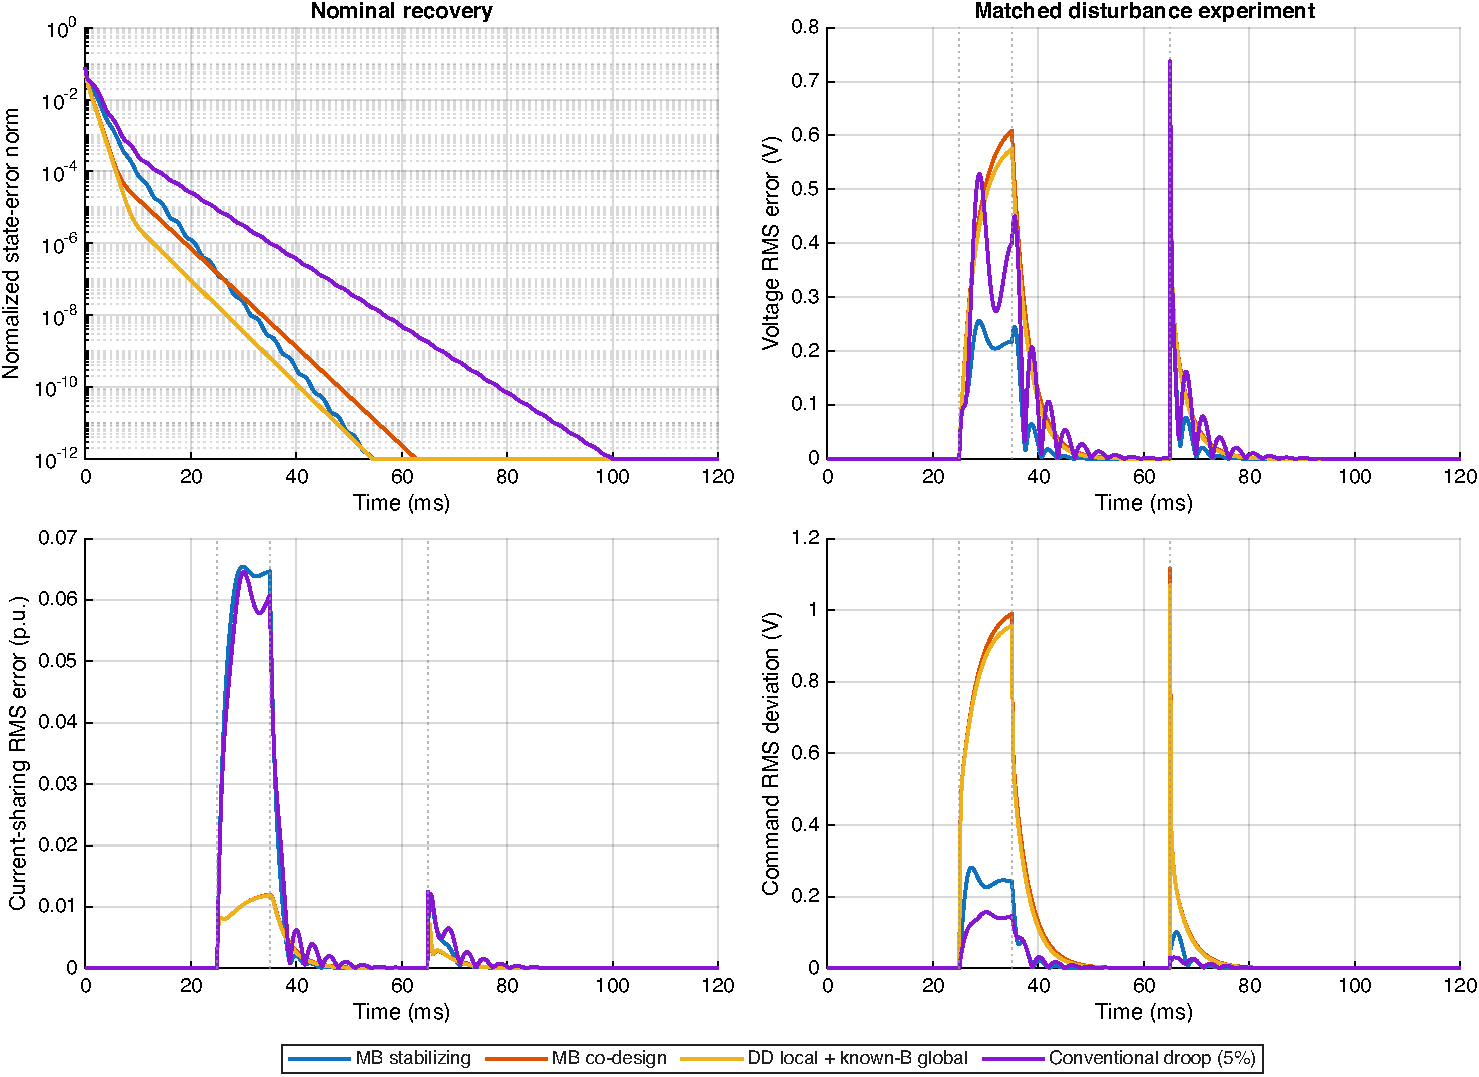
\includegraphics[width=0.86\textwidth]{Results/Regenerated/paper_comparison.pdf}\caption{Nominal recovery and matched disturbance responses. Both voltage tracking and proportional-current-sharing errors are reported, together with controller effort.}\label{Fig:RegeneratedComparison}\end{figure*}
A separate stress experiment varies $L_i,C_i,R_{fi},R_{Li}$ and the constant-current load independently within $\pm10\%$, using a fixed saved seed. Frozen gains are compared with offline MB and DD redesigns on the changed plant (Fig.~\ref{Fig:RegeneratedVariation}). The equilibrium is recomputed for both methods. The DD redesign uses newly collected data and updated known input matrices. This is an empirical parameter-variation study, not a polytopic robustness certificate or an online-adaptation demonstration.
\begin{figure*}[t]\centering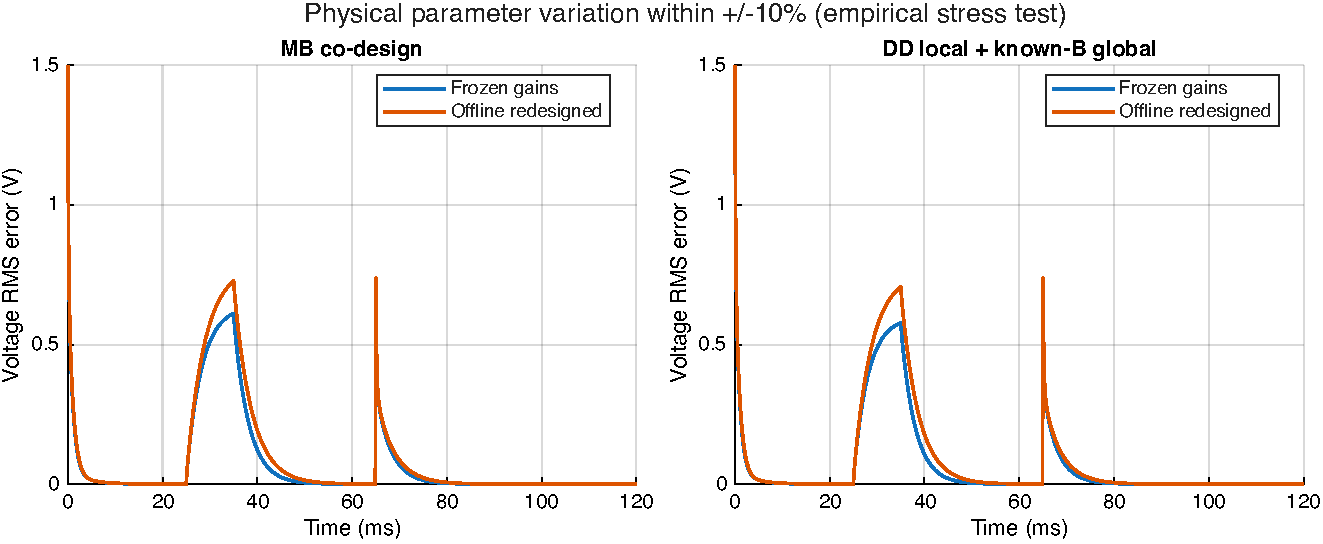
\includegraphics[width=0.86\textwidth]{Results/Regenerated/paper_variation.pdf}\caption{Declared physical-parameter stress experiment, comparing frozen gains and independently verified offline redesigns.}\label{Fig:RegeneratedVariation}\end{figure*}
The complete experiment, including both literature baselines and regression checks, is regenerated by \texttt{run\_all\_paper\_results.m} (also called by \texttt{main.mlx}). The saved records include component values, seeds, data bounds, all tuning attempts, gains, certificates, trajectories, source hashes, and metrics. This run used MATLAB 25.1.0.2943329 (R2025a), YALMIP 20250626, and SEDUMI. Exact propagation agrees with the existing \texttt{DCMicrogrid.dynamics} ODE simulation to $4.50\times 10^{-10}$ in the state infinity norm over the regression interval.
